如图,折线$AOBC$是一段围墙,一根$5$米长的绳子的一端拴在$O$点处的柱子上,另一端拴着一只小狗,

\begin{subquestions}
    \subquestion 请在图中画出小狗的活动区域;
    \subquestion 如果$OA = 6$米,$OB = 3$米,$BC = 5$米,$∠AOB = 90°$,$∠OBC = 120°$,求小狗活动的最大区域的面积.

\end{subquestions}
\begin{center}
    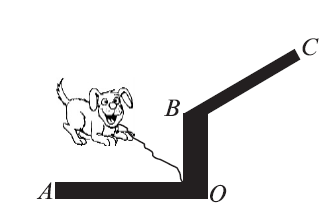
\includegraphics[height=3cm]{lib/image/MJA04040119.png}
\end{center}